\section{Effetti e transizioni}
\subsection{Su liste puntate}
\begin{frame}
  \frametitle{Effetti su liste}
  
  \begin{itemize}
   \item<1-3> Permettono di visualizzare contenuto gradualmente
   \item<2-> Aumentano la attenzione dell'ascoltatore
   \item<4-> L'ordine degli elementi è personalizzabile
   \item<3-> Per farlo si usa \texttt{\textbackslash item}$<n - m>$
   \begin{itemize}
    \item[n] per il numero di click in cui inizierà la transizione
    \item[m] per l'ultimo click in cui sarà visibile la scritta. \\ Facoltativa
   \end{itemize}

  \end{itemize}
  
  
 \begin{textblock*}{5cm}(8.5cm,3cm)
    
\includegraphics[scale=0.15]{magic_wand}
  \end{textblock*}
  
  
 \begin{textblock*}{5cm}(2.8cm,1.2cm)
    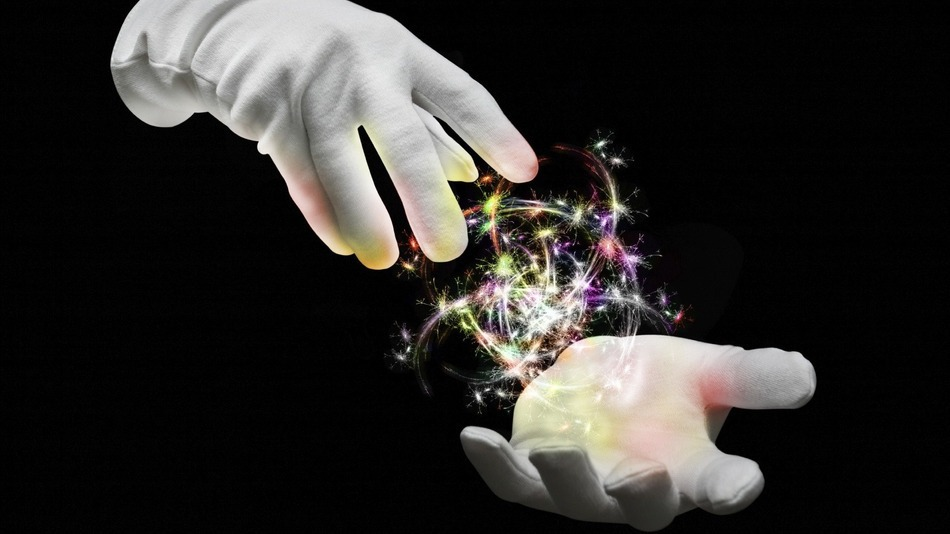
\includegraphics[scale=0.11]{magic}
  \end{textblock*}

\end{frame}
 
